\noindent The first task we face is whether or not we can use machine learning algorithms to 
separate two types of events in a simulated nuclear physics dataset. This being possible
is the minimum requirement a model must meet if we are to apply it to experimental data.
We present the results of training five different models on three simulated 
datasets, as described in section \ref{sec:experimental-background-data}).
Performance is measured using the $F1$ score and confusion matrix. The models range from
the simple logistic regressor, to a deeper CNN architecture with multiple layers. Additionally,
we include a model based on VGG16, as outlined in section \ref{section:method-pretrained},
fine-tuned on simulated data. Somewhat separate from classification, our second objective
is predicting positions of origin and energies associated with events in the dataset.
We follow the same strategy as for classification, with the logistic model replaced by a linear
regressor. The same minimum requirement is valid for regression - models trained on simulated data
must be able to make reasonable predictions. By 'reasonable' we mean 'better than random guessing'.
For this task the performance is measured using the $R2$ score. The variability in results is 
estimated using a K-fold cross-validation approach, with $K = 5$ \cite{Stone1974}.
As a quick recap, the three simulated datasets mentioned are:
\begin{enumerate}[a)]
    \item No changes.
    \item Select pixels set to zero throughout the dataset.
    \item Select pixels set to zero throughout the data, and imbalanced number of single
    and double decays (reduced amount of double decays).
\end{enumerate}

\noindent The machine learning experiments conducted in this thesis were performed
using the AI-Hub computational cluster at the University of Oslo. This resource 
consists of three machines with four RTX 2080 Nvidia GPU’s (graphics
processing unit) each. These cards have ~10GB of memory available for the
allocation of models.

\section{Preliminary analysis}
We begin by looking into the simulated data, more specifically looking for correlations
in the energies and pixel intensities. Note that these results are generated using
dataset (a). In figure \ref{fig:simulated_corrcoeff} we show
the correlation matrix for simulated single and double decays. For single decays, there
is a strong correlation between the energy of the event, the sum of intensities in an image,
and also between the event energy and the intensity of the highest intensity pixel.
The correlation matrix for double events shows similar results. The same, strong correlation
is found for $E1 + E2$ in double decays as for $E1$ in single decays. That is, the total energy
in an event is strongly correlated with the total intensity of pixels in the image.
\begin{figure}
\centering
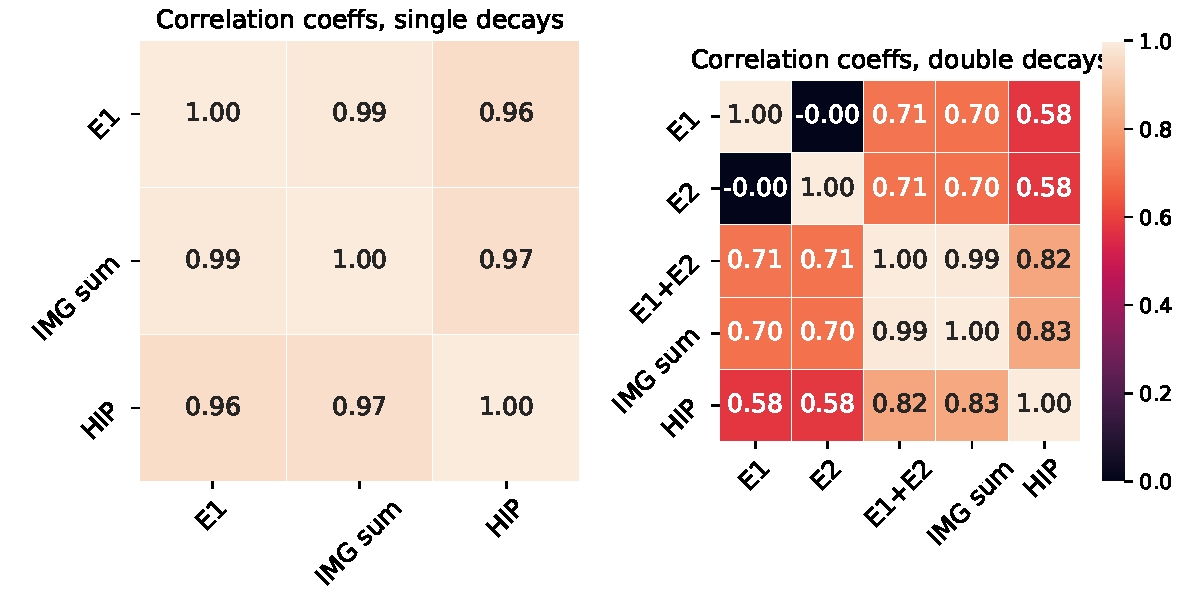
\includegraphics[width=\textwidth]{chapters/results/figures/simulated_corrcoeff.pdf}
\caption{\label{fig:simulated_corrcoeff}Correlation matrices for simulated data,
    separated into single and double decays. $E1$ and $E2$ are the energies corresponding
    to event 1 and event 2 in simulated data. For single events there is no event 2.
    $Sum(image)$ is the sum of all intensities per image in the dataset. HIP is short for
    Highest Intensity Pixel value.
    }
\end{figure}


\noindent Next, we investigate some directly comparable quantities shared by simulated and
experimental data. The distributions of total intensity and highest intensity pixels
in images are shown in figure \ref{fig:comparison-intensity}. 
\begin{figure}
\centering
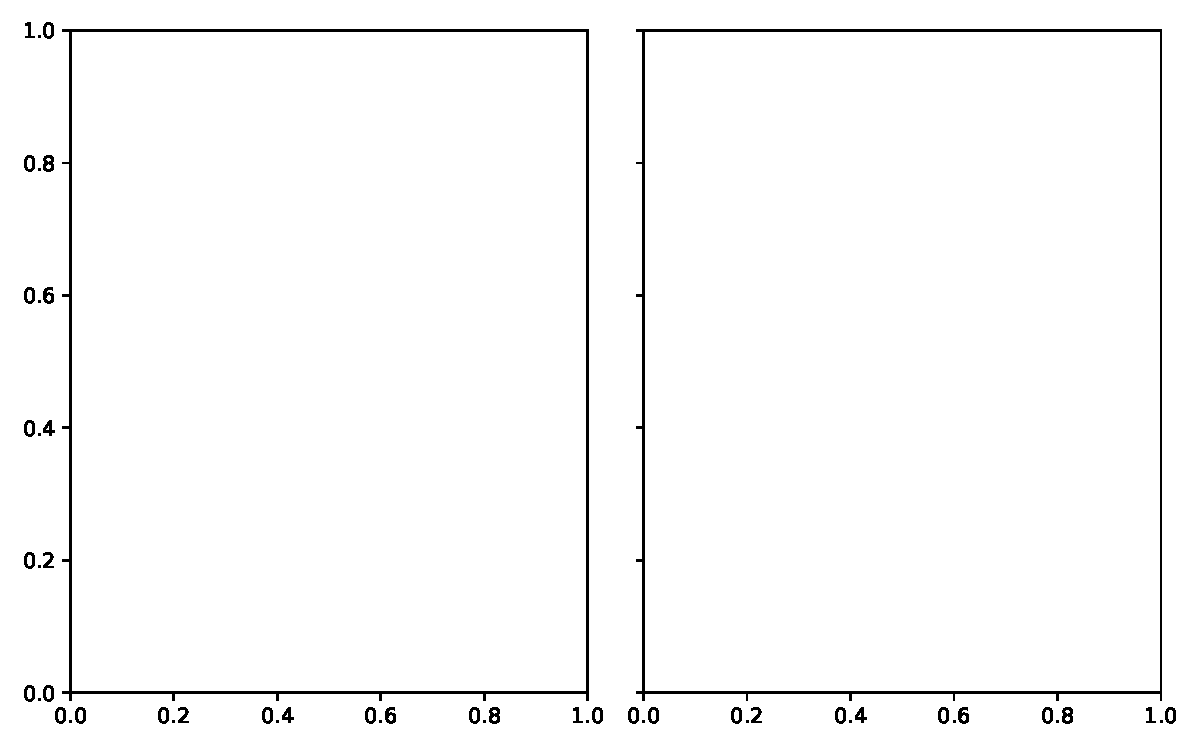
\includegraphics[width=\textwidth]{chapters/results/figures/comparison_intensity.pdf}
\caption{\label{fig:comparison-intensity}Distributions of total pixel intensities and
highest intensities in experimental and simulated decays. Top row compares experimental 
decays and all simulated decays. The bottom row shows the same distributions, but with simulated
decays split into single and double events. The calculations are done post normalization, so
the maximum possible intensity is 1.0.}
\end{figure}
\noindent To relate these distributions more closely to the models themselves, 
the distributions are generated after normalization of the
images. As such, these distributions are what the models 'see'. Looking to the top left
in figure \ref{fig:comparison-intensity} there are a fairly large amount of experimental
decays with higher total intensity than what is present in the simulated data. In the bottom
left plot, it is also clear that there is a point where simulated single and double decays no longer
overlap in total intensities. For the right-hand plots of highest intensity values, there is no such
clear difference between the datasets.
To provide another point of view for this difference, we plot the total intensity in images as
a function of the highest intensity in the images. 
The plot is shown in figure \ref{fig:intensity-hip-comparison}, along with linear fits to the
data.
\begin{figure}
\centering
\includegraphics[width=\textwidth]{chapters/results/figures/intensity_hip_comparison.pdf}
\caption{\label{fig:intensity-hip-comparison}Scatterplot of sum of intensities in images vs
the highest intensity in the same image, for both experimental and simulated decays.
Linear fits give slopes of $a_{experimental}=36.05$ and $a_{simulated}=11.69$.}
\end{figure}
\noindent There is a clear difference between the datasets in that the experimental data
has a higher total intensity. We will come back to these results as we review model
performance on experimental data.

\section{Classification}
\subsection{Classification on simulated data}
In table \ref{tab:classification-simulated-all-f1-auc} the performance of each model
is reported through the estimated $F1$-score, for each of the datasets. 
\begin{table}
\centering
\caption{
Test set F1-scores and roc-AUC scores for classification of simulated datausing multiple models.
Models are trained on a) unmodified data, b) data where specific pixels are set to zero to mimic
'dead' pixels in experimental data, and c) same as b) and imbalanced to mimic experimental data. 
Error estimates are the standard deviation in results from k-fold cross-validation with $K=5$ folds.
}
\label{tab:classification-simulated-all-f1-auc}
\begin{tabular}{llllll}
\toprule
{} &                                            Logistic &                                               Dense &                                       Convolutional &                                    Pretrained VGG16 &                                              Custom \\
\midrule
F1-score (a) &  $\underset{\num{+- 7.727e-03 }  }{\num{ 0.738 } }$ &  $\underset{\num{+- 1.329e-02 }  }{\num{ 0.91 } }$ &  $\underset{\num{+- 6.286e-03 }  }{\num{ 0.964 } }$ &  $\underset{\num{+- 1.591e-02 }  }{\num{ 0.911 } }$ &  $\underset{\num{+- 2.260e-02 }  }{\num{ 0.957 } }$ \\
F1-score (b) &  $\underset{\num{+- 2.273e-03 }  }{\num{ 0.732 } }$ &  $\underset{\num{+- 8.276e-03 }  }{\num{ 0.916 } }$ &  $\underset{\num{+- 3.640e-02 }  }{\num{ 0.758 } }$ &  $\underset{\num{+- 1.926e-02 }  }{\num{ 0.897 } }$ &  $\underset{\num{+- 7.601e-03 }  }{\num{ 0.938 } }$ \\
F1-score (c) &  $\underset{\num{+- 8.483e-02 }  }{\num{ 0.292 } }$ &  $\underset{\num{+- 1.233e-01 }  }{\num{ 0.52 } }$ &  $\underset{\num{+- 9.458e-02 }  }{\num{ 0.9 } }$ &  $\underset{\num{+- 3.606e-02 }  }{\num{ 0.823 } }$ &  $\underset{\num{+- 1.047e-01 }  }{\num{ 0.97 } }$ \\
AUC (a)      &  $\underset{\num{+- 6.515e-04 }  }{\num{ 0.832 } }$ &  $\underset{\num{+- 1.774e-02 }  }{\num{ 0.956 } }$ &  $\underset{\num{+- 2.185e-03 }  }{\num{ 0.988 } }$ &  $\underset{\num{+- 8.505e-03 }  }{\num{ 0.956 } }$ &  $\underset{\num{+- 2.218e-02 }  }{\num{ 0.979 } }$ \\
AUC (b)      &  $\underset{\num{+- 9.779e-04 }  }{\num{ 0.832 } }$ &  $\underset{\num{+- 2.604e-03 }  }{\num{ 0.956 } }$ &  $\underset{\num{+- 9.848e-03 }  }{\num{ 0.977 } }$ &  $\underset{\num{+- 9.530e-03 }  }{\num{ 0.949 } }$ &  $\underset{\num{+- 1.763e-03 }  }{\num{ 0.99 } }$ \\
AUC (c)      &  $\underset{\num{+- 1.601e-03 }  }{\num{ 0.832 } }$ &  $\underset{\num{+- 2.750e-03 }  }{\num{ 0.83 } }$ &  $\underset{\num{+- 8.035e-03 }  }{\num{ 0.944 } }$ &  $\underset{\num{+- 4.376e-03 }  }{\num{ 0.92 } }$ &  $\underset{\num{+- 5.312e-04 }  }{\num{ 0.986 } }$ \\
\bottomrule
\end{tabular}
\end{table}

As a benchmark for transfer learning, we are including a model based on a state of the art pretrained 
network\cite{Simonyan2015}, as outlined in section \ref{sec:method-pretrained}. 
In in figure \ref{fig:confmat-simulated}, we show the confusion matrix for prediction
on test set data for all the models, including normalized values for each event type.
\begin{figure}
\centering
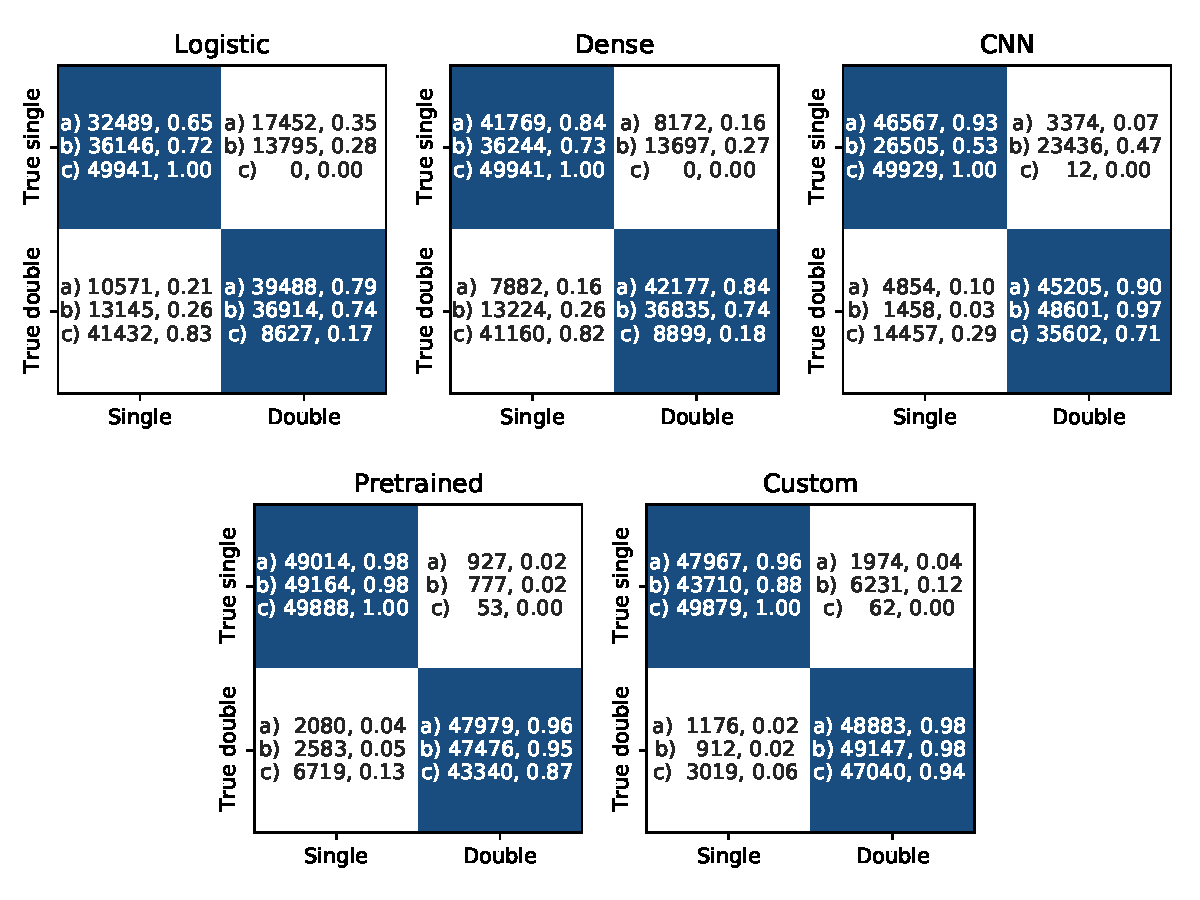
\includegraphics[width=\textwidth]{chapters/results/figures/confmat_simulated.pdf}
\caption{\label{fig:confmat-simulated}Confusion matrices for each model trained
on simulated data. For each model and dataset, the number of events and ratio of each
event type are given. a) unmodified data. b) select pixels set to zero. c) Same as in b)
with the intentionally imbalanced.}
\end{figure}. The F1-scores show decreasing
performance for most models when applying modifications to the unmodified simulated dataset.
When training on an intentionally imbalanced dataset the models without CNN architectures 
show a steep decrease in performance.
Considering the confusion matrix we see that the logistic regressor and dense network
suffer from predicting mostly every sample to be single events. Looking back to the
$F1$-scores again, there is not a significant increase in performance between the
CNN and the Custom model on unmodified data, but the custom model performs strongly
across all datasets, with a low amount of misclassified events relative to the other
models. Again looking at the confusion matrices (figure \ref{fig:confmat-simulated}),
Double decays are more often misclassified as single than the opposite.
Next, we apply the 'classifiers' to experimental data.

\subsection{Classification on experimental data}
Classification of experimental data poses a different set of challenges when it comes
to evaluating our results. We currently only have a small number of events that are
hand labelled as double events, which may be used as a form of verification. As mentioned in section
\ref{sec:experimental-background}, we expect the number of double events in the experimental
data to be much lower than single events. Inspecting the ratio of predicted singles to predicted
doubles can then be an initial indication of how a model is performing. It is, however,
not conclusive. Correctly classified hand labelled events are another indication, but
is also not conclusive. In table \ref{tab:classification-experimental-ratios}, the ratios
of predicted singles to predicted doubles are presented for each model trained on each
dataset. The actual number of predictions for each class are included below the ratios.
\begin{table}
\centering
\caption{
Decay event classification on experimental data, with models trained on:
a) unmodified data, b) data where specific pixels are set to zero to mimic
'dead' pixels in experimental data, and c) same as b) and imbalanced to mimic experimental data.
}
\label{tab:classification-experimental-ratios}
\begin{tabular}{lllllll}
\toprule
{} &                                     Single (a) &                                     Double (a) &                                     Single (b) &                                     Double (b) &                                     Single (c) &                                     Double (c) \\
\midrule
Logistic   &  $\underset{\num{ 198210 }  }{\num{ 0.762 } }$ &  $\underset{\num{ 61937 }  }{\num{ 0.238 } }$ &  $\underset{\num{ 202426 }  }{\num{ 0.778 } }$ &  $\underset{\num{ 57721 }  }{\num{ 0.222 } }$ &  $\underset{\num{ 260145 }  }{\num{ 1.000 } }$ &  $\underset{\num{ 2 }  }{\num{ 0.000 } }$ \\
Dense      &  $\underset{\num{ 97487 }  }{\num{ 0.375 } }$ &  $\underset{\num{ 162660 }  }{\num{ 0.625 } }$ &  $\underset{\num{ 100778 }  }{\num{ 0.387 } }$ &  $\underset{\num{ 159369 }  }{\num{ 0.613 } }$ &  $\underset{\num{ 260122 }  }{\num{ 1.000 } }$ &  $\underset{\num{ 25 }  }{\num{ 0.000 } }$ \\
CNN        &  $\underset{\num{ 63051 }  }{\num{ 0.242 } }$ &  $\underset{\num{ 197096 }  }{\num{ 0.758 } }$ &  $\underset{\num{ 66790 }  }{\num{ 0.257 } }$ &  $\underset{\num{ 193357 }  }{\num{ 0.743 } }$ &  $\underset{\num{ 98594 }  }{\num{ 0.379 } }$ &  $\underset{\num{ 161553 }  }{\num{ 0.621 } }$ \\
Pretrained &  $\underset{\num{ 138614 }  }{\num{ 0.533 } }$ &  $\underset{\num{ 121533 }  }{\num{ 0.467 } }$ &  $\underset{\num{ 137765 }  }{\num{ 0.530 } }$ &  $\underset{\num{ 122382 }  }{\num{ 0.470 } }$ &  $\underset{\num{ 259448 }  }{\num{ 0.997 } }$ &  $\underset{\num{ 699 }  }{\num{ 0.003 } }$ \\
Custom     &  $\underset{\num{ 26277 }  }{\num{ 0.101 } }$ &  $\underset{\num{ 233870 }  }{\num{ 0.899 } }$ &  $\underset{\num{ 24738 }  }{\num{ 0.095 } }$ &  $\underset{\num{ 235409 }  }{\num{ 0.905 } }$ &  $\underset{\num{ 52951 }  }{\num{ 0.204 } }$ &  $\underset{\num{ 207196 }  }{\num{ 0.796 } }$ \\
\bottomrule
\end{tabular}
\end{table}

Overall there is a strong preference for classifying events as double decays. This makes
the validation using hand labelled doubles in table \ref{tab:classification-experimental-labeled-doubles}
somewhat moot, since it is hard to attribute these 'correct' classifications to the models'
ability to recognize the double decays.
\begin{table}
\centering
\caption{
Decay event classification on 17 labeled samples of experimental data. The 17 samples are all
labeled as double events. Models are trained on simulated data with a varying degree of modification:
a) unmodified data, b) data where specific pixels are set to zero to mimic
'dead' pixels in experimental data, and c) same as b) and imbalanced to mimic experimental data.
The numbers are shown as the normalized ratio of predicted event type, with the actual amount of
events predicted of that type below.
}
\label{tab:classification-experimental-labeled-doubles}
\begin{tabular}{lllllll}
\toprule
{} &                                Single (a) &                                 Double (a) &                                Single (b) &                                 Double (b) &                                Single (c) &                                 Double (c) \\
\midrule
Logistic   &  $\underset{\num{ 0 }  }{\num{ 0.000 } }$ &  $\underset{\num{ 17 }  }{\num{ 1.000 } }$ &  $\underset{\num{ 0 }  }{\num{ 0.000 } }$ &  $\underset{\num{ 17 }  }{\num{ 1.000 } }$ &  $\underset{\num{ 1 }  }{\num{ 0.059 } }$ &  $\underset{\num{ 16 }  }{\num{ 0.941 } }$ \\
Dense      &  $\underset{\num{ 0 }  }{\num{ 0.000 } }$ &  $\underset{\num{ 17 }  }{\num{ 1.000 } }$ &  $\underset{\num{ 0 }  }{\num{ 0.000 } }$ &  $\underset{\num{ 17 }  }{\num{ 1.000 } }$ &  $\underset{\num{ 0 }  }{\num{ 0.000 } }$ &  $\underset{\num{ 17 }  }{\num{ 1.000 } }$ \\
CNN        &  $\underset{\num{ 0 }  }{\num{ 0.000 } }$ &  $\underset{\num{ 17 }  }{\num{ 1.000 } }$ &  $\underset{\num{ 0 }  }{\num{ 0.000 } }$ &  $\underset{\num{ 17 }  }{\num{ 1.000 } }$ &  $\underset{\num{ 0 }  }{\num{ 0.000 } }$ &  $\underset{\num{ 17 }  }{\num{ 1.000 } }$ \\
Pretrained &  $\underset{\num{ 0 }  }{\num{ 0.000 } }$ &  $\underset{\num{ 17 }  }{\num{ 1.000 } }$ &  $\underset{\num{ 0 }  }{\num{ 0.000 } }$ &  $\underset{\num{ 17 }  }{\num{ 1.000 } }$ &  $\underset{\num{ 3 }  }{\num{ 0.176 } }$ &  $\underset{\num{ 14 }  }{\num{ 0.824 } }$ \\
Custom     &  $\underset{\num{ 0 }  }{\num{ 0.000 } }$ &  $\underset{\num{ 17 }  }{\num{ 1.000 } }$ &  $\underset{\num{ 0 }  }{\num{ 0.000 } }$ &  $\underset{\num{ 17 }  }{\num{ 1.000 } }$ &  $\underset{\num{ 0 }  }{\num{ 0.000 } }$ &  $\underset{\num{ 17 }  }{\num{ 1.000 } }$ \\
\bottomrule
\end{tabular}
\end{table}

\begin{figure}
\centering
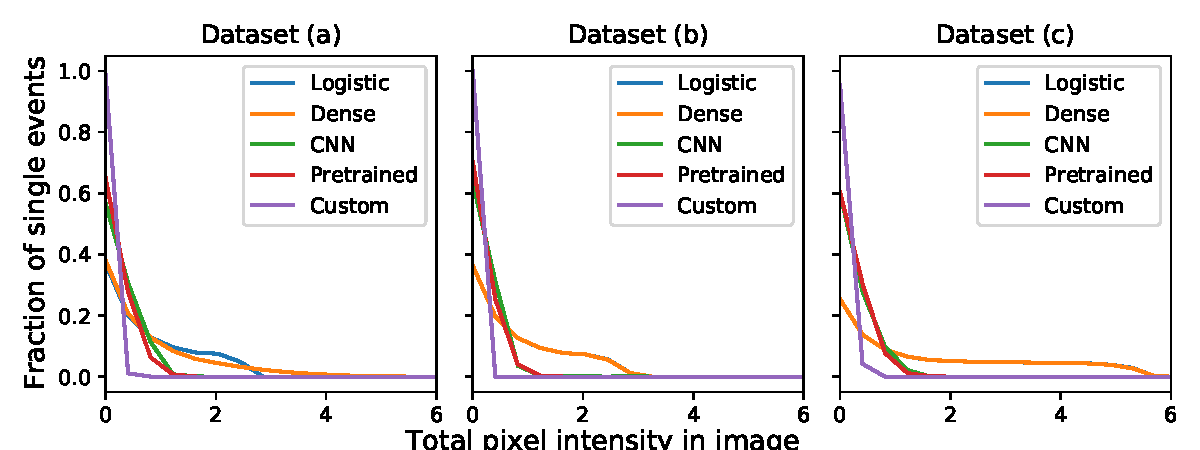
\includegraphics[width=\textwidth]{chapters/results/figures/classification_experimental_single_fractions.pdf}
\caption{\label{fig:experimental-single-fractions}Fraction of predicted singles as a function of
total intensity in images, for each model trained on simulated data.  a) unmodified data. b) select pixels set to zero. 
c) Same as in b) with the intentionally imbalanced.}
\end{figure}
As the number of events is large, manual inspection of each predicted class is not feasible.
In figure \ref{fig:experimental-single-fractions} we show the fraction of predicted single events
in experimental data as a function of total intensity in each image. Regardless of which simulated
dataset a model is trained on, the majority of  single events are predicted at low total intensites.
The only exception to this is the Dense model trained on dataset $c$. Keep in mind, however, that the
total intensities for experimental data span from 0 to ~18 (see figure \ref{fig:comparison-intensity}).
To further prod this apparent trend, we perform a simple test using the Custom model trained on dataset $b$.
For a set of single events for which we know the model has good performance, we multiply the image intensities
with a scaling factor from 0-10. The aim is to see the effect of increasing total intensity in
images on the classification accuracy. The result is shown in figure \ref{fig:simulated-scaled-intensities}.
\begin{figure}
\centering
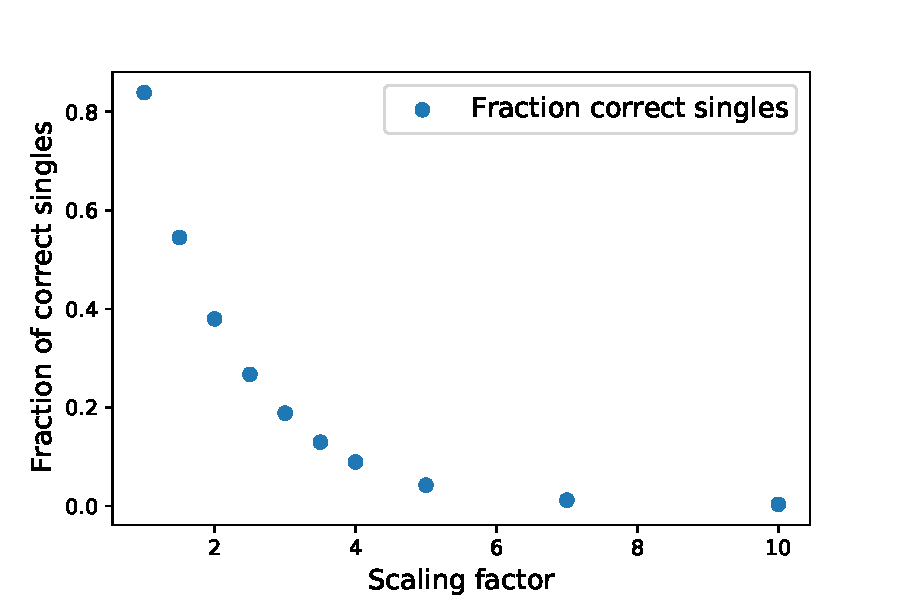
\includegraphics[width=\textwidth]{chapters/results/figures/simulated_scaled_intensity.pdf}
\caption{\label{fig:simulated-scaled-intensities}Fraction of simulated single events correctly classified
as a function of scaling factor used to increase the total intensity in simulated
decays. The model used for classification is the Custom model trained on dataset (b),
which has select pixels set to zero.}
\end{figure}
From this figure, there is a clear trend towards a lower fraction of events correctly classified as single 
decays when the intensities in images increases. Note that at a scaling factor of 4 the total intensities in
the simulated images approach the highest total intensities in the experimental decay data.
 
\section{Regression}
Assuming data has already been classified, we aim to predict the energy of the decays and their
position of origin. Because there is a travel distance between the 
ejection site and the point the energy is deposited, the positions aren't necessarily
the locations of the highest-intensity pixels in the detector images. Our hypothesis is
then that there are sufficient structures and spacial relationships in the detector images to
allow a model to determine these positions.
Note that for regression the models are trained on single or double events exclusively.
A consequence of this is that for dataset $c$ the set of single events is
identical to that of set $b$, causing near-identical results between these two sets.

\subsection{Position of origin}
In table \ref{tab:regression-simulated-all-positions-r2} the R2-scores for all models
trained on simulated data are presented.
\begin{table}
\centering
\caption{
Test set R2-scores for regression of positions of origin on simulated data, with models trained on data with: 
a) no modifications, b) specific pixels set to zero to mimic experimental data, and c) imbalanced dataset
in addition to modifications in b) to further mimic experimental data. Error estimates are the standard deviation 
in results from validation data in k-fold cross-validation with $K=5$ folds.
}
\label{tab:regression-simulated-all-positions-r2}
\begin{tabular}{llllll}
\toprule
{} &                                              Linear &                                               Dense &                                                 CNN &                                           Pretrained &                                              Custom \\
\midrule
Single (a) &  $\underset{\num{+- 2.889e-03 }  }{\num{ 0.8 } }$ &  $\underset{\num{+- 7.007e-04 }  }{\num{ 0.988 } }$ &  $\underset{\num{+- 9.207e-04 }  }{\num{ 0.997 } }$ &  $\underset{\num{+- 2.229e-01 }  }{\num{ 0.997 } }$ &  $\underset{\num{+- 1.366e-04 }  }{\num{ 0.999 } }$ \\
Single (b) &  $\underset{\num{+- 2.749e-03 }  }{\num{ 0.781 } }$ &  $\underset{\num{+- 1.406e-03 }  }{\num{ 0.982 } }$ &  $\underset{\num{+- 1.110e-03 }  }{\num{ 0.98 } }$ &  $\underset{\num{+- 4.513e-04 }  }{\num{ 0.997 } }$ &  $\underset{\num{+- 9.603e-04 }  }{\num{ 0.995 } }$ \\
Single (c) &  $\underset{\num{+- 2.749e-03 }  }{\num{ 0.781 } }$ &  $\underset{\num{+- 1.424e-03 }  }{\num{ 0.982 } }$ &  $\underset{\num{+- 1.080e-03 }  }{\num{ 0.98 } }$ &  $\underset{\num{+- 4.932e-04 }  }{\num{ 0.997 } }$ &  $\underset{\num{+- 1.639e-03 }  }{\num{ 0.993 } }$ \\
Double (a) &  $\underset{\num{+- 3.766e-03 }  }{\num{ 0.37 } }$ &  $\underset{\num{+- 5.601e-03 }  }{\num{ 0.456 } }$ &  $\underset{\num{+- 1.603e-03 }  }{\num{ 0.471 } }$ &  $\underset{\num{+- 1.552e-01 }  }{\num{ 0.29 } }$ &  $\underset{\num{+- 3.467e-04 }  }{\num{ 0.493 } }$ \\
Double (b) &  $\underset{\num{+- 6.815e-04 }  }{\num{ 0.364 } }$ &  $\underset{\num{+- 3.431e-03 }  }{\num{ 0.458 } }$ &  $\underset{\num{+- 1.835e-03 }  }{\num{ 0.435 } }$ &  $\underset{\num{+- 1.550e-01 }  }{\num{ 0.289 } }$ &  $\underset{\num{+- 2.865e-04 }  }{\num{ 0.489 } }$ \\
Double (c) &  $\underset{\num{+- 7.768e-03 }  }{\num{ 0.357 } }$ &  $\underset{\num{+- 9.456e-03 }  }{\num{ 0.417 } }$ &  $\underset{\num{+- 2.507e-03 }  }{\num{ 0.442 } }$ &  $\underset{\num{+- 8.452e-01 }  }{\num{ -0.924 } }$ &  $\underset{\num{+- 4.187e-03 }  }{\num{ 0.478 } }$ \\
\bottomrule
\end{tabular}
\end{table}

\noindent A similar trend as was seen for classification
can be observed for single events, where models are trained on unmodified data. Even
a linear regressor predicts positions of origin fairly well, but it is clear
that the neural networks perform at a much higher level in this case. They have strong
R2-scores of 0.99 and higher, and very little degradation in performance with added 
modifications to the training data. Again, as with classification, the custom model
performs strongly across all datasets for single events, with the lowest variability across
experiments. However, in this regression task, the pretrained model.
In the case of regression on double events, none of the models accurately
predict positions of origins for both events.
\begin{table}
\centering
\caption{
Mean distances of predicted position of origin on experimental data, to center of highest intensity pixel (HIP).Models 
trained on data with: a) no modifications, b) specific pixels set to zero to mimic experimental data, and c) imbalanced dataset
in addition to modifications in b) to further mimic experimental data.
}
\label{tab:regression-experimental-dist-means}
\begin{tabular}{ll}
\toprule
{} & Mean distance [mm] \\
\midrule
LinReg (a)     &  $\num{ 19.19 }$ \\
Dense (a)      &  $\num{ 63.27 }$ \\
CNN (a)        &  $\num{ 10.72 }$ \\
Pretrained (a) &  $\num{ 17.52 }$ \\
Custom (a)     &  $\num{ 13.23 }$ \\
LinReg (b)     &  $\num{ 19.97 }$ \\
Dense (b)      &  $\num{ 32.06 }$ \\
CNN (b)        &  $\num{ 11.92 }$ \\
Pretrained (b) &  $\num{ 16.43 }$ \\
Custom (b)     &  $\num{ 4.39 }$ \\
LinReg (c)     &  $\num{ 19.97 }$ \\
Dense (c)      &  $\num{ 32.04 }$ \\
CNN (c)        &  $\num{ 11.85 }$ \\
Pretrained (c) &  $\num{ 16.43 }$ \\
Custom (c)     &  $\num{ 7.08 }$ \\
\bottomrule
\end{tabular}
\end{table}

In the absence of true positions for experimental decays, we rely on other
ways to estimate how regression models perform.
\begin{figure}
\centering
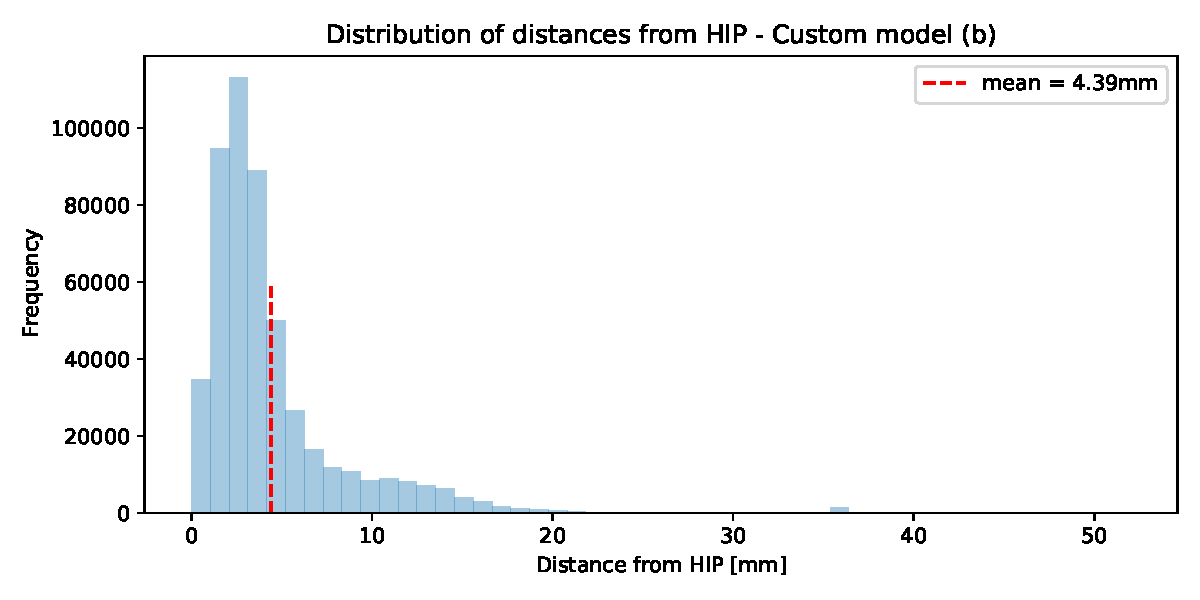
\includegraphics[width=\textwidth]{chapters/results/figures/experimental_pos_dist.pdf}
\caption{\label{fig:experimental-pos-dist} Distribution of distances between predicted
positions of origin and the highest intensity pixel(HIP) in the corresponding images. 
The model was a custom cnn architecture, trained on simulated data where (b) denotes 
that elect pixels were set to zero across the dataset. This model was selected for this
plot due to it having the lowest mean distance from HIP.}
\end{figure}
In figure \ref{fig:experimental-pos-dist} we look at how the predicted positions
are distributed around the highest intensity pixel in each experimental decay event.
As a comparison, we plot the same distribution using true values for positions in
simulated single decay events. We can see that the distributions overlap quite well
up until their respective peaks. Predictions on experimental decays have a wider
distribution than the target data, but as we've seen in the classification results this
difference in distributions is not a unique case.

\subsubsection{Energy}
In table \ref{tab:regression-simulated-all-energies-r2} we show the R2-scores for all
models trained on simulated data.
Performance when predicting single energies is across the board lower than what we saw
for positions of origin. On unmodified data, the models are to a large degree able to
predict energies, with R2-scores of 0.93 and above. For the modified datasets the CNN
suffers greatly and isn't able to account for variances in the data at all. Other models
see a less severe effect, but still a clear reduction in the goodness of fit.
As was the case with the prediction of positions, no models predict energies
of double events with any useful degree of accuracy.
\begin{table}
\centering
\caption{
Test set R2-scores for regression of energies on simulated data, with models trained on data with: 
a) no modifications, b) specific pixels set to zero to mimic experimental data, and c) imbalanced dataset
in addition to modifications in b) to further mimic experimental data. Error estimates are the standard deviation 
in results from validation data in k-fold cross-validation with $K=5$ folds.
}
\label{tab:regression-simulated-all-energies-r2}
\begin{tabular}{llllll}
\toprule
{} &                                              Linear &                                               Dense &                                                 CNN &                                          Pretrained &                                              Custom \\
\midrule
Single (a) &  $\underset{\num{+- 3.334e-02 }  }{\num{ 0.932 } }$ &  $\underset{\num{+- 3.623e-02 }  }{\num{ 0.934 } }$ &  $\underset{\num{+- 4.088e-02 }  }{\num{ 0.937 } }$ &  $\underset{\num{+- 3.761e-02 }  }{\num{ 0.926 } }$ &  $\underset{\num{+- 2.997e-02 }  }{\num{ 0.944 } }$ \\
Single (b) &  $\underset{\num{+- 2.459e-02 }  }{\num{ 0.768 } }$ &  $\underset{\num{+- 2.222e-02 }  }{\num{ 0.745 } }$ &  $\underset{\num{+- 2.575e-02 }  }{\num{ 0.48 } }$ &  $\underset{\num{+- 1.948e-02 }  }{\num{ 0.781 } }$ &  $\underset{\num{+- 3.167e-02 }  }{\num{ 0.752 } }$ \\
Single (c) &  $\underset{\num{+- 2.459e-02 }  }{\num{ 0.768 } }$ &  $\underset{\num{+- 2.223e-02 }  }{\num{ 0.745 } }$ &  $\underset{\num{+- 2.522e-02 }  }{\num{ 0.432 } }$ &  $\underset{\num{+- 1.955e-02 }  }{\num{ 0.781 } }$ &  $\underset{\num{+- 2.956e-02 }  }{\num{ 0.724 } }$ \\
Double (a) &  $\underset{\num{+- 3.349e-02 }  }{\num{ 0.49 } }$ &  $\underset{\num{+- 3.084e-02 }  }{\num{ 0.49 } }$ &  $\underset{\num{+- 4.130e-02 }  }{\num{ 0.488 } }$ &  $\underset{\num{+- 3.138e-02 }  }{\num{ 0.489 } }$ &  $\underset{\num{+- 3.618e-02 }  }{\num{ 0.491 } }$ \\
Double (b) &  $\underset{\num{+- 3.157e-03 }  }{\num{ 0.485 } }$ &  $\underset{\num{+- 2.347e-03 }  }{\num{ 0.487 } }$ &  $\underset{\num{+- 7.096e-03 }  }{\num{ 0.478 } }$ &  $\underset{\num{+- 4.508e-03 }  }{\num{ 0.489 } }$ &  $\underset{\num{+- 3.659e-03 }  }{\num{ 0.464 } }$ \\
Double (c) &  $\underset{\num{+- 4.611e-02 }  }{\num{ 0.434 } }$ &  $\underset{\num{+- 4.583e-02 }  }{\num{ 0.422 } }$ &  $\underset{\num{+- 4.554e-02 }  }{\num{ 0.446 } }$ &  $\underset{\num{+- 3.868e-02 }  }{\num{ 0.417 } }$ &  $\underset{\num{+- 4.802e-02 }  }{\num{ 0.401 } }$ \\
\bottomrule
\end{tabular}
\end{table}


Due to the poor performance of models trained on simulated double events, and the
expected low frequency of double events in the experimental data, we only apply models
trained on simulated single events. From figure \ref{fig:simulated_corrcoeff}, we know
that total image intensity and energy are closely correlated for simulated data,
and from $R2$ scores shown in table \ref{tab:regression-simulated-all-energies-r2}
that goodness of fit decreases with added 'dead' pixels. Without true values for
energies in experimental data, we show in figure \ref{fig:regression-energy-intensity-prediction-energy-zeros}
the related quantities for experimental decays. Total image intensity decreases with
increasing number of pixels with value zero, as expected. The predicted energy
follows this same trend very closely. The 'peaks' in the plots correspond to events
where there are a fairly large amount of 'dead' pixels, but the decay was registered
in a region of the detector with few such pixels.
\begin{figure}
\centering
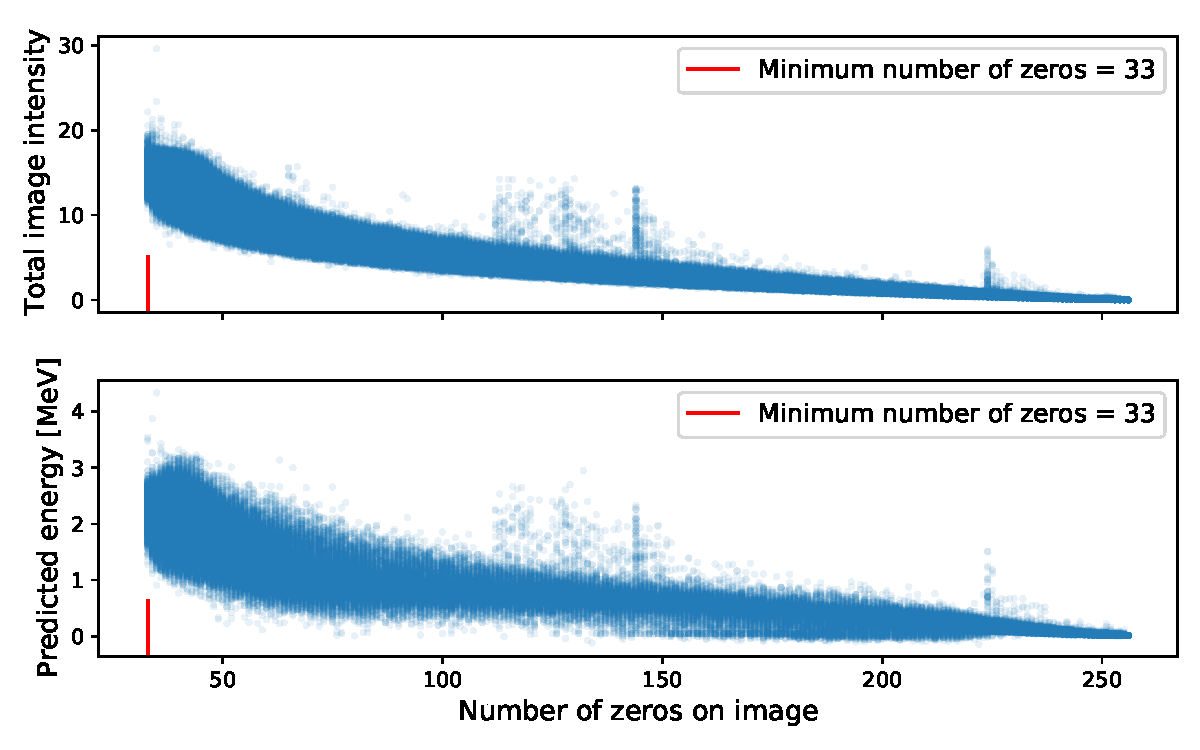
\includegraphics[width=\textwidth]{chapters/results/figures/tot_intensity_predicted_energy_vs_zeros.pdf}
    \caption{\label{fig:regression-energy-intensity-prediction-energy-zeros} 
    Top: Total image intensities as a function of number of pixels with 
    intensity zero in images. Bottom: Predicted energy for experimental
    decays events as a function of number of pixels with intensity zero 
    in images. The model used for predictions is the Custom architecture model
    trained on dataset $b$.}
\end{figure}

We also calculate the correlation coefficients between total image intensity and
predicted energy for all models applied to experimental data. For all models the
correlation coefficients range from 0.95 to 0.999.
